\section{Product Perspective}
The core of SafeStreets is the opportunity to create a community that cooperates to reduce traffic violations: for this to be possible, it is necessary to integrate third party services with our software. 
Our software works with the APIs provided by Google Maps to best help the users identify the location of the violation they want to report.
We also work with different municipalities that help us provide better statistics by sharing with us their data about traffic violations, so our software needs to interact with their APIs and reduce the differences in communication standards as much as possible.
In order to encourage citizens to become SafeStreets users, we will create partnerships with different brands. Through these partnerships we will be able to send prizes to users that contribute the most to the community.

\begin{figure}[H]
  \centering
  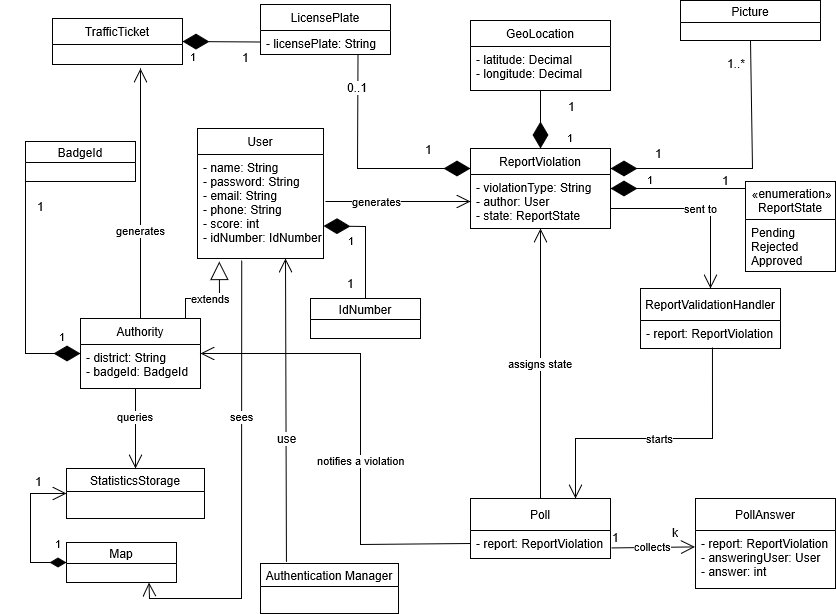
\includegraphics[width=\textwidth]{RASD_Images/uml.jpg}
  \caption{\textit{UML class diagram}}
\end{figure}

\begin{figure}[H]
  \centering
  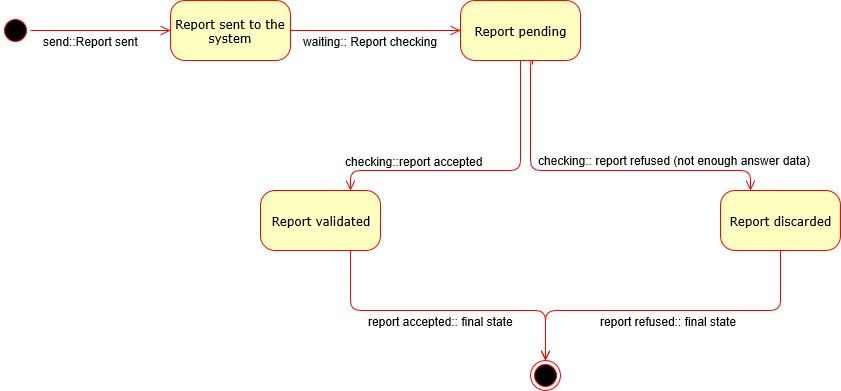
\includegraphics[width=\textwidth]{RASD_Images/StateDiagrams/state1.jpg}
  \caption{\textit{State diagram 1 - Report}}
\end{figure}

\begin{figure}[H]
  \centering
  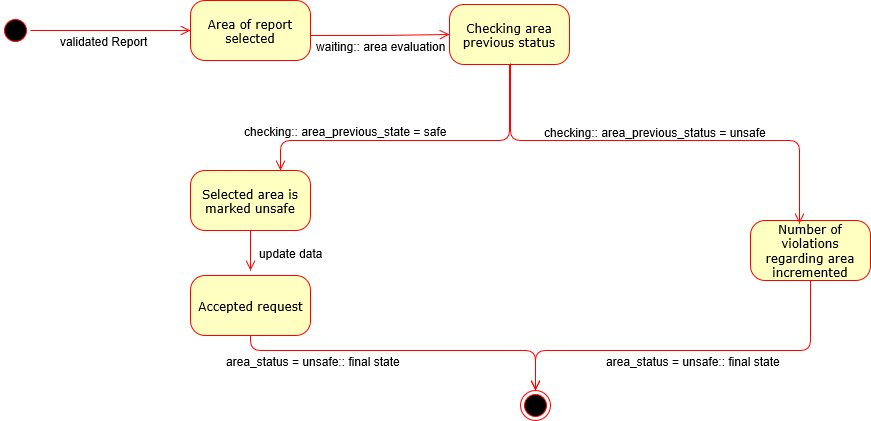
\includegraphics[width=\textwidth]{RASD_Images/StateDiagrams/state2.jpg}
  \caption{\textit{State diagram 2 - Area}}
\end{figure}

\begin{figure}[H]
  \centering
  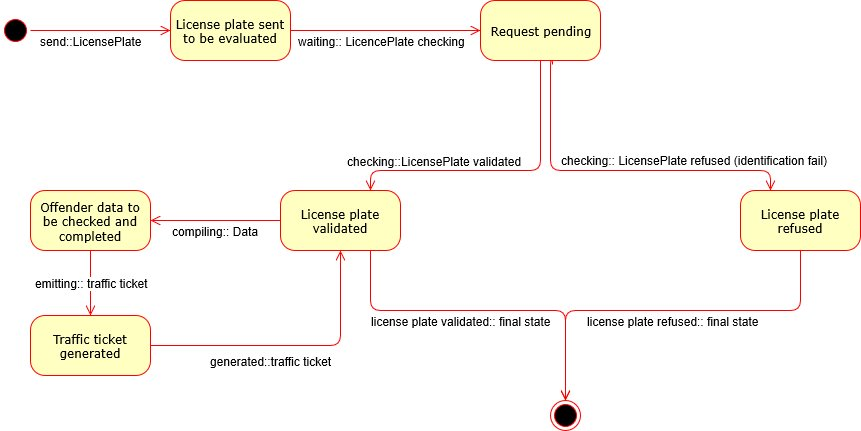
\includegraphics[width=\textwidth]{RASD_Images/StateDiagrams/state3.jpg}
  \caption{\textit{State diagram 3 - License plate}}
\end{figure}

\begin{figure}[H]
  \centering
  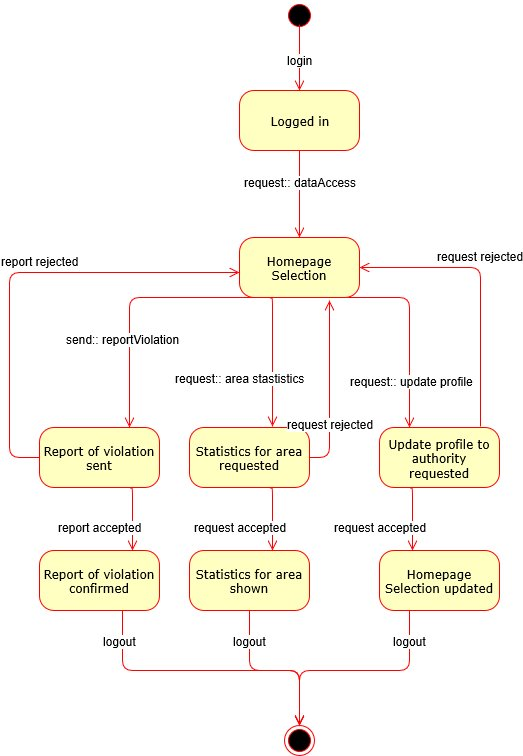
\includegraphics[width=7 cm]{RASD_Images/StateDiagrams/state4.jpg}
  \caption{\textit{State diagram 4 - User login}}
\end{figure}
